% $Author$ $Date$
% from \Chapter{average}{13nov2006}{Averaging}

\subsection{Energy budget} % of the \KSe}
\label{sec:energy}

% Predrag                   mar 13 2007
%
\PC{As nobody else deigns to do it, I picked the low fruit that I have been talking about past month: defined the energy input and energy dissipation rates for Kuramoto-Sivashinsky. I cannot believe that it is not in the literature, it is standard energy balance exercise vor Navier Stokes case. This should show the isolated equilibria far from the chaotic measures, and the important rpos well embedded in it. More importantly, if Loss gives us Sobolev bounds on energy, we might be able to bound the number of equilibria as function of systems size L, and thus be sure we have them all.
   }
%
The {\em space average} of a quantity $\obser$ that may depend
on the point $x$ of phase space $\pS$ and on the time $t$ is given
by the $d$-dimensional integral over the $d$ coordinates of the
dynamical system:
\bea
	\expct{a}\!(t) & = & {1\over |\pS|} \intM{x} \obser(x(t))
   	\continue
	|\pS| &=& \intM{x} = \mbox{\rm volume of~}\pS
	\,.
	\label{rpo:spac_ave}
\eea
The space $\pS$ is assumed to have finite dimension and volume.

The {\em time average} of the observable
along a trajectory is defined by
\index{averaging!time}
\beq
	\timeAver{\obser(\xInit)} 
	= 
	\lim_{t\rightarrow \infty} {1\over t} 
	\int_0^t d\tau \, \obser(\flow{\tau}{\xInit})
	\,.
\ee{rpo:tim_ave}

The time average
$\timeAver{\obser(\xInit)}$ takes a particularly simple form when
evaluated on a periodic orbit. Define
\beq
         \obser_p = \frac{1}{\period{p}}
  \int_0^{\period{p} } \obser\left(\flow{\tau}{\xInit} \right)d\tau 
\,,
\hspace{1.0cm}  \xInit \in p
\,,
\label{rpo:Phi_cyc}
\eeq
where $p$ is a prime cycle, $\period{p}$ is its period,
$\obser_p$ is a loop integral of the observable
along a single parcourse of a prime cycle $p$, so it is an intrinsic
property of the cycle,  independent of the starting point $\xInit \in p$.
Evaluation of the infinite time average \refeq{rpo:tim_ave} requires 
only a single traversal of the cycle.

Let us define 
the {\em expectation value}
$\expct{\obser}$ of an observable $\obser$ to be the asymptotic time
and space average over the phase space $\pS$
\beq
	\expct{\obser}  = 
	\lim_{t\rightarrow \infty} {1\over |\pS|} 
	\intM{x}
		{1\over t} \int_0^t d\tau \,
		\obser(\flow{\tau}{x})
	\,.
\ee{rpo:s_tim_ave}
We use the same $\expct{\cdots}$ notation as for
the space average \refeq{rpo:spac_ave}, and distinguish
the two by the presence of the time variable in the argument: if
the quantity $\expct{a}\!(t)$ being averaged depends on time, then it is a 
space
average, if it does not, it is the expectation value $\expct{\obser}$.

Take time derivative of the mean energy \refeq{ksEnergy},
substitute \refeq{ks} and integrate by parts. Total derivatives vanish
by the spatial periodicity on the $L$ domain:
\bea
   \frac{1}{2}\dot{E} &=& \frac{1}{L}\int_0^{L}u \, u_t\, dx
	 = \expct{u (u^2)_x}(t) - \expct{u \, u_{xx}}(t) 
	   - \expct{u \, u_{xxxx}}(t)
	\continue
	&=&
- \expct{ u_x \, u^2}(t)
+ \expct{u_{x}^2}(t)
- \expct{u_x \, u_{xxx}}(t)
    \,.
\label{rpo:ksErate}
\eea
For an equilibrium it follows from \refeq{KSeqvCond}
that $E$ is constant, as it should be:
\[
   \frac{1}{2}\dot{E} = 
\expct{ u_x \,(-u^2 + u_{x} - u_{xxx})}(t)
	= - \expct{ u_x }E =0
    \,.
\]
The first term in \refeq{rpo:ksErate} vanishes by
integration by parts,
\beq
0=
\expct{ u_x \, u^2}+ \expct{u (u^2)_x} 
= 
\expct{ u_x \, u^2}+ 2 \expct{u^2\,u_x} 
\,,
\ee{EnNonl0}
and integrating by parts yet again the third term we get
that the energy rate\PC{this is ``power", nicht war?}
\beq
   \frac{1}{2}\dot{E}(t) = 
	  \expct{u_{x}^2}(t) - \expct{u_{xx}^2}(t)
\ee{EnRate}
is the balance between energy pumped in by the anti-diffusion
term $u_{xx}$ and burned up by hypervicosity $u_{xxxx}$
in KS equation \refeq{ks}.

In \reffig{f:drivedrag}
we plot drive $\expct{u_{x}^2}(t)$ vs. 
dissipation $\expct{u_{xx}^2}(t)$ for all $L=22$ \eqva\
and \reqva, several \po s and \rpo s, and for a typical ``turbulent"
evolution. Notice that the single \rpo\ with $T\simeq32$ captures a large
part of the turbulent dynamics \ES{Momentarilly adopting Japanese philosophy,
before putting there the rest of the short orbits.}.

%%%%%%%%%%%%%%%%%%%%%%%%%%%%%%%%%%%%%%%%%%%%%%%%%%%%%%%%%%%%%%%%
\begin{figure}[t] \label{f:drivedrag}
\begin{center}
	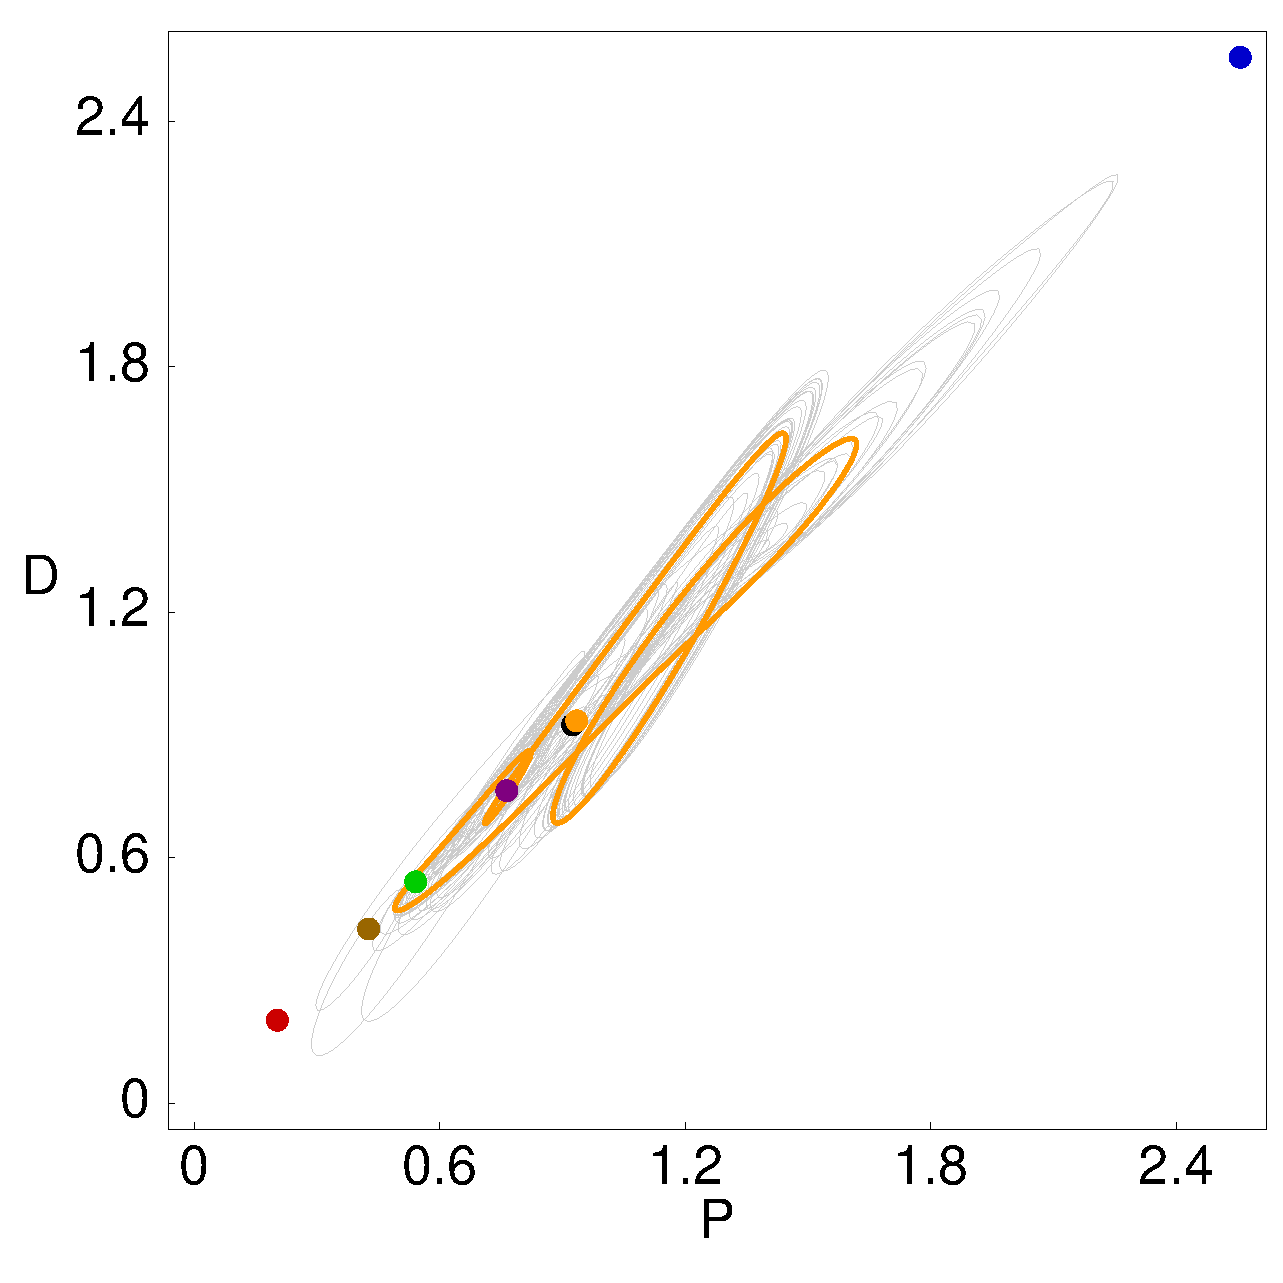
\includegraphics[width=\textwidth]{figs/energyBalancePlot.eps}
\end{center}
\caption{
Energy input $\expct{u_{x}^2}(t)$ vs. 
dissipation $\expct{u_{xx}^2}(t)$ for all $L=22$ \eqva\
and \reqva, several (two, more in the way!) \po s and \rpo s, and for a typical ``turbulent"
evolution. Note the isolation of the \eqva\ which do not participate in
chaotic dynamics (?).
        }
\end{figure}
%%%%%%%%%%%%%%%%%%%%%%%%%%%%%%%%%%%%%%%%%%%%%%%%%%%%%%%%%%%%%%%%%%


The time average $\timeAver{E}$
computed on arbitrary orbit goes to a constant, so
the expectation values \refeq{rpo:EtimAve} of drive and dissipation
exactly balance each out:
\beq
	0= \timeAver{\dot{E}}  = 
	\lim_{t\rightarrow \infty}
		{1\over t} \int_0^t d\tau \, \dot{E}(\tau)
=
	  \expct{u_{x}^2} - \expct{u_{xx}^2}
	\,.
\ee{rpo:EtimAve}
In particular, the \eqva\
and \reqva\ sit on the diagonal in \reffig{f:drivedrag},
and so do time-averages computed on \po s and \rpo s:
\bea
E_p &=& 
{1\over \period{p}} \int_0^\period{p}d\tau \, E(\tau)
	\continue
\expct{u_{x}^2}_p &=& 
{1\over \period{p}} \int_0^\period{p} d\tau \, \expct{u_{xx}^2} (\tau)
	=
	  \expct{u_{xx}^2}_p
	\,.
\label{poE}
\eea
[STILL TO TYPE IN: $\expct{u^2}(t) =$ Fourier space norm, etc.]
%
\PC{Next: Michael Loss will teach us how to bound $E$ by
    Sobolev bounds}
\PC{Next for fluid guys: Read LIeb and Ruelle to learn
    how to bound $E$ for plane Couette by Sobolev bounds}
